\documentclass{article}
\usepackage{fontspec}

% Used to embed Sage code in latex
%\usepackage{sagetex}


% Math Environment
\usepackage{euler}        % Euler font
\usepackage{amsmath}      % Math macros
\usepackage{amssymb}      % Math symbols
\usepackage{unicode-math} % Unicode support

% Physics Environment
\usepackage{physics}


\usepackage[makeroom]{cancel} % Used to cancel terms in algebraic equations
\usepackage{ulem} % Different underline environments
\usepackage{polynom} %Polynomial long division

% Typesetting Rules
\setlength\parindent{0em}
\setlength\parskip{0.618em}
\usepackage[a4paper,lmargin=1in,rmargin=1in,tmargin=1in,bmargin=1in]{geometry}
\setmainfont[Mapping=tex-text]{Helvetica Neue LT Std 45 Light}

% Common Macros
\newcommand\N{\mathbb{N}}
\newcommand\Z{\mathbb{Z}}
\newcommand\Q{\mathbb{Q}}
\newcommand\R{\mathbb{R}}
\newcommand\C{\mathbb{C}}
\newcommand\A{\mathbb{A}}
\def\res{\mathop{\text{Res}}\limits}

% Color
\usepackage[dvipsnames]{xcolor}
\usepackage{pagecolor}
% \definecolor{DeepMossGreen}{HTML}{394820}
% \pagecolor{DeepMossGreen}
% \color{Goldenrod}

\usepackage{graphicx}

\begin{document}

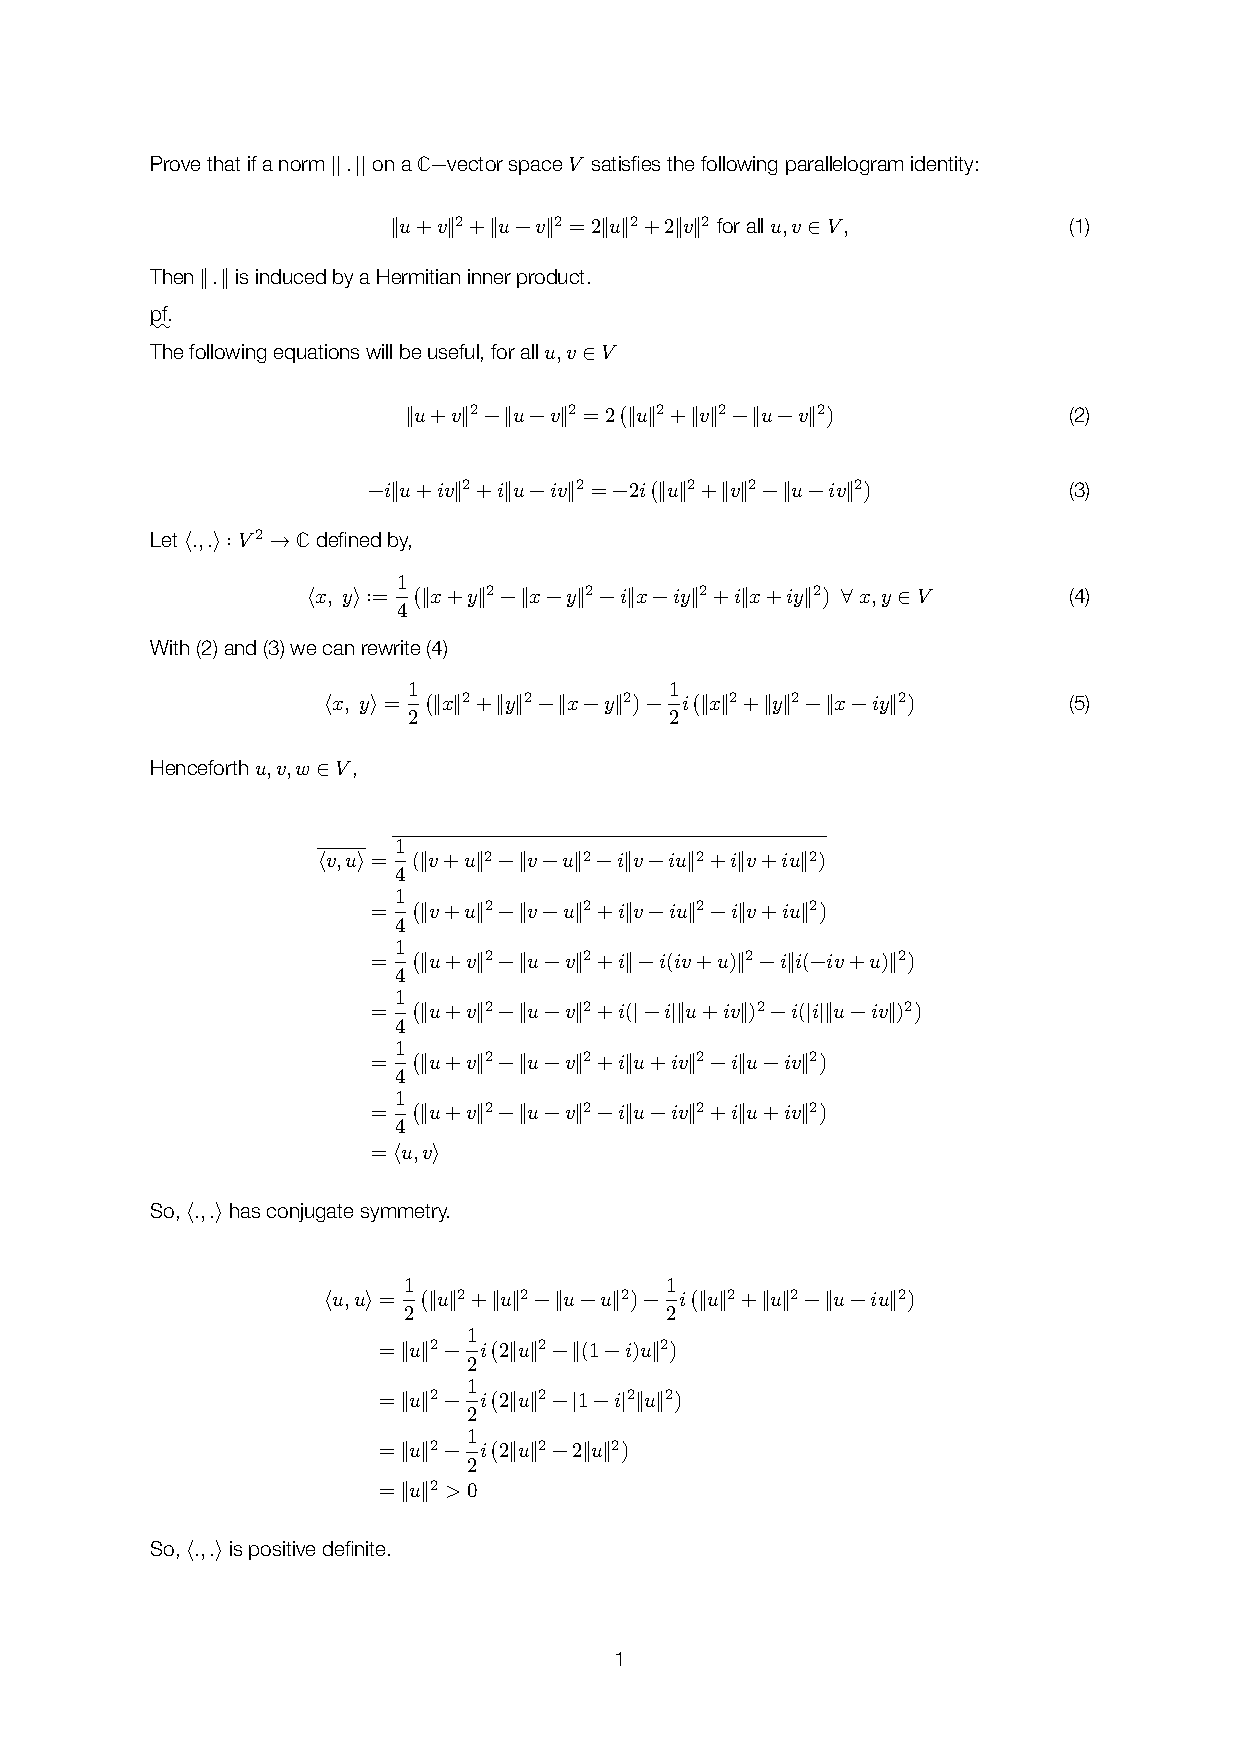
\includegraphics[width=\textwidth]{q1.png}

\uwave{slu.}

Consider $f:\R^2\rightarrow\R;(x,y)\mapsto e^x-e^y\cos(y)$

$f(0,0) = 0$

$[f'(x,y)]  = \begin{pmatrix} e^x & e^y\sin(y) -e^y\cos(y)\end{pmatrix}$

det$([f'(x,y)]_{x})  = e^x \neq 0 $


Since, $\cos(y)$ is periodic $f$ is not injective.

$f$ is not surjective since $e^x$ is non-negative, and $-1
<-e^y\cos(y)< 1$, so $\forall (x,y)\in \R^2 -1<f(x,y).$

So, $f$ cannot
define a in implicit function $g:\R\rightarrow \R$ such that $g$ satisfies,
$f(g(y),y) = 0,\quad \forall y\in \R\quad \blacklozenge$

\end{document}




%%% Local Variables:
%%% mode: latex
%%% TeX-master: t
%%% End:
